\documentclass[10pt]{article}  % list options between brackets
\usepackage{etex}
\usepackage[italian]{babel} % Adatta LaTeX alle convenzioni tipografiche italiane
\usepackage[utf8]{inputenc} % Consente l'uso dei caratteri accentati italiani
\usepackage{mdframed} %per mettere delle box attorno a qualsiasi cosa
\usepackage{graphicx} % Per le immagini
\usepackage {fancyhdr} % Per l' ambiente abstract
\usepackage{indentfirst} % Indentazione all' inizio dei capitoli
\usepackage{url} % Formattazione URL
\usepackage{amsmath} % Vari simboli matematici
\usepackage{amssymb} %Per l' "uguale per definizione"
\usepackage{amsthm} % Per le dimostrazioni
\usepackage{amsfonts} % Per font matematici
\usepackage{mathrsfs} % Per i font corsivi belli, tipo la N delle gaussiane ecc...
\usepackage{listings} % Per il codice
\usepackage{easybmat} % Per le matrici a blocchi
\usepackage{mathtools}
\usepackage{color}
\usepackage{tikz}
\usepackage{syntax}
\usetikzlibrary{trees}
\newcommand{\fncyblank}{\fancyhf{}} %
\frenchspacing % Non aumentare la spaziatura tra periodi
\newcommand{\footnoteremember}[2] % Accesso multiplo a note a pie' pagina
{
    \footnote{#2}
    \newcounter{#1}
    \setcounter{#1}
    {
        \value{footnote}
    }
}
\newcommand{\footnoterecall}[1]
{
    \footnotemark[\value{#1}]
}

\lstdefinelanguage{JavaScript}{
  keywords={typeof, new, true, false, catch, function, return, null, catch, switch, var, if, in, while, do, else, case, break},
  ndkeywords={class, export, boolean, throw, implements, import, this},
  sensitive=false,
  comment=[l]{//},
  morecomment=[s]{/*}{*/},
  morestring=[b]',
  morestring=[b]"
}

\begin{document}
\title{TCPSG\\Estensione SSL}   % type title between braces
\author{Cosimo Sacco, Davide Silvestri}         % type author(s) between braces
\date{}    % type date between braces
\maketitle
\begin{abstract}
    L'estensione illustrata aggiunge la funzionalità di SSL acceleration al port tcpsg.
\end{abstract}
\section{Il port TCPSG}
    \label{sec:tcpsg}
    Tcpsg è un semplice TCP port forwarder.
    Il programma gestisce ciascuna connessione da parte di un cliente affidandola ad un nuovo processo servente.
    \begin{lstlisting}[language=C]
        if (child_count < main_opt.max_clients)
        {
            if((pid = fork()) == 0){...}
            .
            .
            .
        }
    \end{lstlisting}
    Il processo principale rimane in ascolto di nuove richieste.
    \begin{lstlisting}[language=C]
connfd = accept( listenfd, (struct sockaddr *) NULL, NULL);
    \end{lstlisting}
    Il processo servente si connette al server.
    \begin{lstlisting}[language=C]
server_sockfd = connect_to(serv_address, serv_portno);
    \end{lstlisting}
    Il processo servente entra in un ciclo ed effettua la select sul descrittore relativo al server e su quello relativo al client.
    \begin{lstlisting}[language=C]
FD_SET(server_sockfd, &frwd_fds);
FD_SET(client_sockfd, &frwd_fds);
select(FD_SETSIZE, &frwd_fds, NULL, NULL, NULL);
    \end{lstlisting}

    Quando un descrittore è pronto per la lettura, effettua il forwarding del traffico fra server e client utilizzando un buffer di appoggio.
    \begin{lstlisting}[language=C]
if (FD_ISSET(client_sockfd, &frwd_fds))
{
    /* Read from client and write to server... */
    if((nbytes = recv(client_sockfd, frwd_buffer, BUFFER_SIZE, 0)) < 1)
        return(nbytes);
    if ((nbytes = send(server_sockfd, frwd_buffer, nbytes, 0)) < 1)
        return(nbytes);
}
    \end{lstlisting}

\section{SSL accelerator}
    L'utilizzo di \emph{SSL} garantisce la \emph{confidenzialità}, \emph{integrità}
    ed \emph{autenticità} (opzionalmente sul server) dei dati trasmessi.

    Le operazioni di \emph{apertura del canale SSL}, di \emph{cifratura} e di \emph{decifratura}
    risultano particolarmente onerose.
    In particolare, è preferibile sollevare il server dall'onere di effettuare le suddette operazioni,
    relegando le stesse ad un componente esterno detto \emph{SSL accelerator}.
    Solitamente l'SSL accelerator ed il processo server risiedono sulla stessa rete locale
    o sono comunque collegati attraverso un mezzo ritenuto sicuro, mentre il client e l'SSL accelerator
    comunicano attraverso un canale SSL.
\section{Implementazione}
    \subsection{OpenSSL Wrapper}
    Al fine di semplificare l'utilizzo delle API di OpenSSL, e quindi rendere il codice prodotto
    il più compatto possibile, abbiamo realizzato il seguente \emph{wrapper layer}:
        \begin{lstlisting}[language=C]
typedef struct
{
    SSL* ssl;
    SSL_CTX* ctx;
} SSLSocket;

SSLSocket* SSLOpen(int baseSocket, char* keyFile, char* password, char* caFile);

inline int SSLAccept(SSLSocket* secureSocket);

inline int SSLConnect(SSLSocket* secureSocket);

inline int SSLRead(SSLSocket* secureSocket, void* buffer, int bufferSize);

inline int SSLGetError(SSLSocket* secureSocket, int err);

inline int SSLWrite(SSLSocket* secureSocket, void* buffer, int bufferSize);

int checkCertificate(SSLSocket* secureSocket, char* hostname);

void SSLClose(SSLSocket* secureSocket);
        \end{lstlisting}
        Il layer maschera tutte le operazioni di inizializzazione e gestione del canale,
        offrendo un'interfaccia simile a quella dei socket.
        \begin{figure}[htbp]
            \centering
            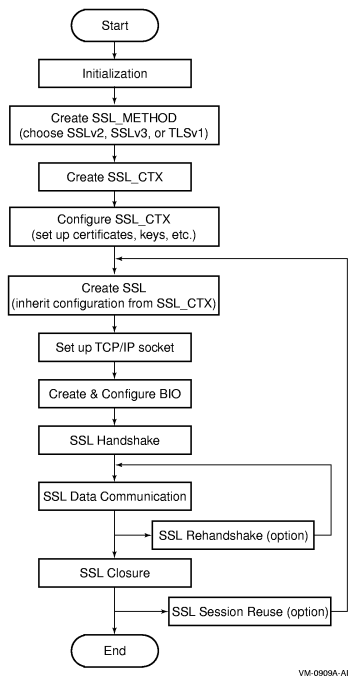
\includegraphics[scale=0.45]{ssl.png}
            \caption{\emph{Flow chart}, OpenSSL API}
        \end{figure}
    \subsection{Modifica di tcpsg}
        La modifica da noi effettuata permette di stabilire un canale sicuro con il
        client direttamente sul port forwarder. In questo modo non è necessario che il
        server si occupi di gestire la sicurezza del canale.

        Abbiamo modificato il file di configurazione in modo che sia possibile attivare SSL:
        \begin{lstlisting}[language=Bash]
# This is the configuration file used by tcpsg
# this is a sample file working like a telnet gateway
# with two servers


# The local port where the gateway listen requests from clients

localport 2300

# The server port where the real servers will listen request from gateway

serverport 23

# The number of clients simultaneously connected to the gateway

maxclients 10

# The servers ip address, you must use the order to specify the priority
# used to select each server. The first server in the list has the highest
# priority and the last has the lowest priority.

server 127.0.0.1

# If 1 enables SSL connection between client and tcpsg.

sslflag 1

# Keyfile contains server certificate and private key.

keyfile server.pem

# Keyfile password.

password abcd
        \end{lstlisting}
        Alla ricezione di una richiesta da parte di un client, se il flag SSL è stato settato,
        viene invocato l'handler da noi implementato.
        \begin{lstlisting}[language=C]
if (main_opt.sslflag)
{
if(secureRedirect(connfd, main_opt.serverhost[server_id], &main_opt.serverport) < 0)
    writemsg("Failed to attempt to redirect data");
}
        \end{lstlisting}
        L'handler gestore si connette al server e si occupa di negoziare i parametri crittografici per la creazione
        del canale sicuro verso il client:
        \begin{lstlisting}[language=C]
if((serverSocket = connect_to(serv_address, serv_portno)) < 0)
return serverSocket;
.
.
.
secureSocket = SSLOpen(clientSocket, main_opt.keyfile, main_opt.password, NULL);
if(secureSocket == NULL) return -1;
        \end{lstlisting}
        In seguito si mette in attesa di scritture da parte del server o del client:
        \begin{lstlisting}[language=C]
FD_SET(server_sockfd, &frwd_fds);
FD_SET(client_sockfd, &frwd_fds);
select(FD_SETSIZE, &frwd_fds, NULL, NULL, NULL);
        \end{lstlisting}
        Alla ricezione di dati da parte del server, l'handler provvede a redirigerli
        sul canale sicuro verso il client:
        \begin{lstlisting}[language=C]
// Read from server and secure write to client...
if( (nbytes = recv(serverSocket, buffer, BUFFER_SIZE, 0)) < 1){...}
error = SSLWrite(secureSocket, buffer, nbytes);
if(error != SSL_ERROR_NONE){...}
        \end{lstlisting}
        Viceversa, alla ricezione sul canale sicuro di dati provenienti dal client,
        l'handler provvede alla redirezione in chiaro verso il server:
        \begin{lstlisting}[language=C]
// Secure read from client and write to server...
nbytes = SSLRead(secureSocket, buffer, BUFFER_SIZE);
error = SSLGetError(secureSocket,nbytes);
if(error != SSL_ERROR_NONE){...}
if((nbytes = send(serverSocket, buffer, nbytes, 0)) < 1 ){...}
        \end{lstlisting}
    \subsection{Testing}
        Per il test dell'applicazione abbiamo realizzato un semplice server
        ed un client SSL che si scambiano delle stringhe.
        I certificati \emph{X509} e le coppie di chiavi pubblica/privata sono
        stati generati attraverso l'utilizzo del tool \texttt{openssl}.
\end{document}
